% 2x2 framework diagram crossing Novelty x Specificity, where each cell
% contains a mini three-column (Intensity x Item x Outcome) breakdown
% drawn in the same style as exposure_outcome_diagram.tex, plus the
% three count lines (pairings / primary outcomes / pooled estimates).
%
%   Rows:    Novelty     (No: overall availability | Yes: new introductions)
%   Columns: Specificity (No: general meat sales   | Yes: counterpart-specific sales)
%
% Each cell's mini-diagram:
%   A1: {Count, Proportion}    x {Analog-Modifiable, Vegan, Vegetarian}        x {6 general sales}     fully crossed
%   A2: {Presence, Count}      x {6 analog types}                              x {6 counterpart sales} 1-to-1 matched
%   A3: {New Introduction}     x {Analog-Modifiable, Vegan, Vegetarian}        x {6 general sales}     fully crossed
%   A4: {New Introduction}     x {6 analog types}                              x {6 counterpart sales} 1-to-1 matched
%
% Build with:  tectonic publication/novelty_specificity_expanded_diagram.tex

\documentclass[border=10pt, tikz]{standalone}

\usepackage{tikz}
\usetikzlibrary{positioning, decorations.pathreplacing, calc, arrows.meta, fit}

\begin{document}
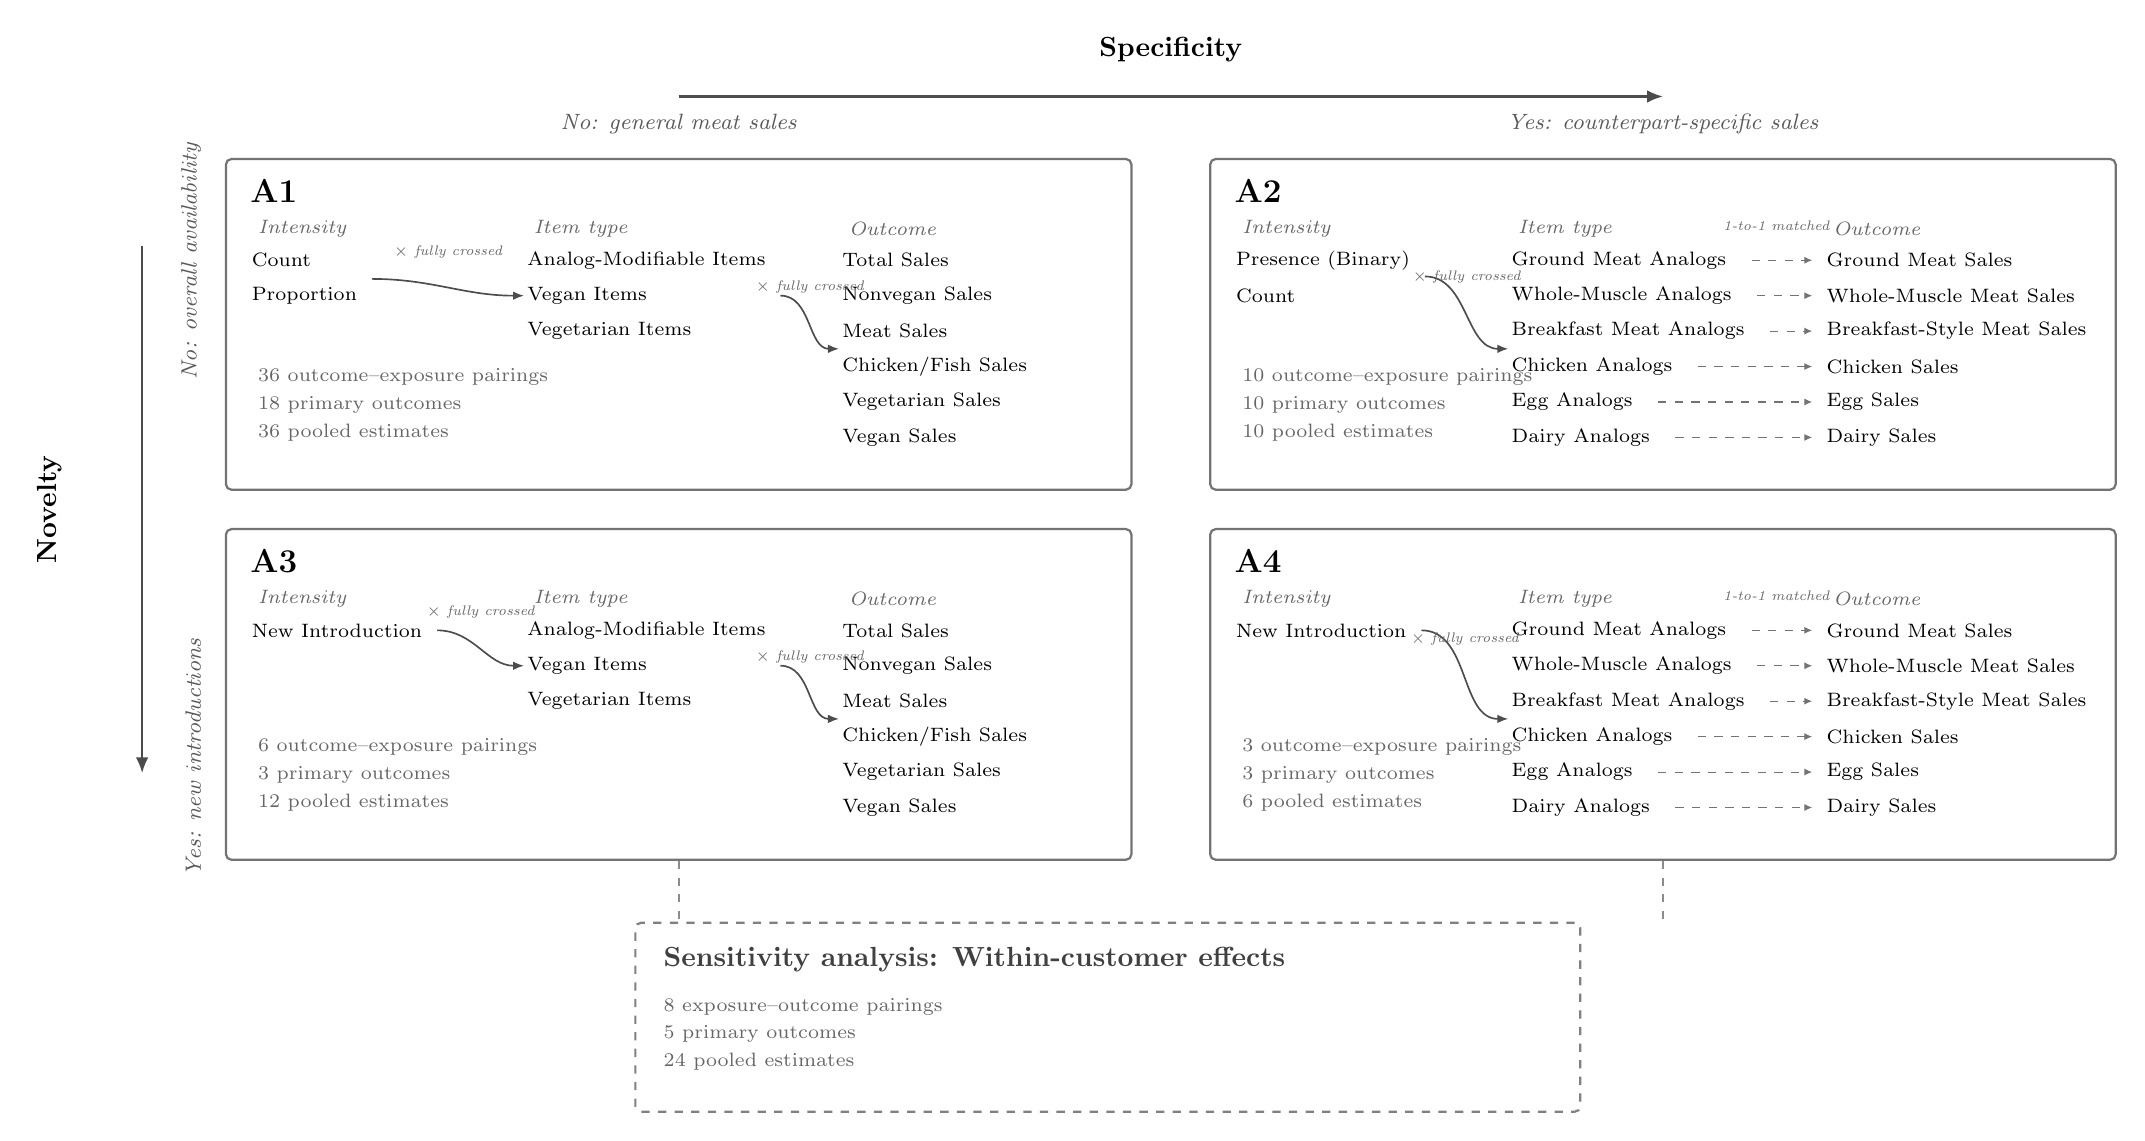
\begin{tikzpicture}[
  font=\small,
  axis label/.style  = {font=\bfseries},
  level/.style       = {font=\itshape\footnotesize, text=black!65},
  cell/.style        = {draw=black!55, thick, rounded corners=2pt,
                        minimum width=115mm, minimum height=42mm,
                        anchor=north west},
  ccell/.style       = {draw=black!50, thick, dashed, rounded corners=2pt,
                        minimum width=120mm, minimum height=24mm,
                        align=left, inner sep=7pt, anchor=north west},
  alabel/.style      = {font=\bfseries\large},
  clabel/.style      = {font=\bfseries, text=black!75},
  subhead/.style     = {font=\itshape\scriptsize, anchor=west, text=black!60},
  miniitem/.style    = {font=\scriptsize, anchor=west, inner sep=1pt},
  countline/.style   = {font=\scriptsize, text=black!60, anchor=north west},
  arr/.style         = {-{Latex[length=2.0mm,width=1.6mm]},
                        thick, color=black!70},
  miniarr/.style     = {-{Latex[length=1.4mm,width=1.1mm]},
                        semithick, color=black!70},
  minimatch/.style   = {-{Latex[length=1.0mm,width=0.9mm]}, dashed,
                        color=black!55, shorten >=4pt, shorten <=8pt},
  minicross/.style   = {font=\itshape\tiny, color=black!60},
  lead/.style        = {dashed, thick, color=black!45},
]

% =============================================================
% Grid cells (2 x 2)
% =============================================================
\node[cell] (A1) at (0.0,   0.0) {};
\node[cell] (A2) at (12.5,  0.0) {};
\node[cell] (A3) at (0.0,  -4.7) {};
\node[cell] (A4) at (12.5, -4.7) {};

% Within each cell (anchored from north-west):
%   A# label  at -0.15
%   subhead   at -0.90  (above items)
%   items     start at -1.30, step -0.45
%   count1    at -3.90
%   count2    at -4.25
%   count3    at -4.60

% --- A1: no novelty, no specificity ---
\node[alabel, anchor=north west] at ($(A1.north west)+(0.20,-0.15)$) {A1};

\coordinate (A1c1) at ($(A1.north west)+(0.30,-1.30)$);
\coordinate (A1c2) at ($(A1.north west)+(3.80,-1.30)$);
\coordinate (A1c3) at ($(A1.north west)+(7.80,-1.30)$);

\node[subhead] at ($(A1c1)+(0,0.40)$) {Intensity};
\node[subhead] at ($(A1c2)+(0,0.40)$) {Item type};
\node[subhead] at ($(A1c3)+(0,0.40)$) {Outcome};

\node[miniitem] (A1c1r1) at (A1c1)              {Count};
\node[miniitem] (A1c1r2) at ($(A1c1)+(0,-0.45)$) {Proportion};

\node[miniitem] (A1c2r1) at (A1c2)               {Analog-Modifiable Items};
\node[miniitem] (A1c2r2) at ($(A1c2)+(0,-0.45)$) {Vegan Items};
\node[miniitem] (A1c2r3) at ($(A1c2)+(0,-0.90)$) {Vegetarian Items};

\node[miniitem] (A1c3r1) at (A1c3)               {Total Sales};
\node[miniitem] (A1c3r2) at ($(A1c3)+(0,-0.45)$) {Nonvegan Sales};
\node[miniitem] (A1c3r3) at ($(A1c3)+(0,-0.90)$) {Meat Sales};
\node[miniitem] (A1c3r4) at ($(A1c3)+(0,-1.35)$) {Chicken/Fish Sales};
\node[miniitem] (A1c3r5) at ($(A1c3)+(0,-1.80)$) {Vegetarian Sales};
\node[miniitem] (A1c3r6) at ($(A1c3)+(0,-2.25)$) {Vegan Sales};

\node[fit=(A1c1r1)(A1c1r2), inner xsep=4pt, inner ysep=1pt] (A1c1box) {};
\node[fit=(A1c2r1)(A1c2r3), inner xsep=4pt, inner ysep=1pt] (A1c2box) {};
\node[fit=(A1c3r1)(A1c3r6), inner xsep=4pt, inner ysep=1pt] (A1c3box) {};

% Arrows land at the middle of the next column.
\coordinate (A1arr2end) at ($(A1c3r3.west)!0.5!(A1c3r4.west)$);
\draw[miniarr] (A1c1box.east) to[out=0, in=180] (A1c2r2.west);
\draw[miniarr] (A1c2box.east) to[out=0, in=180] (A1arr2end);

\node[minicross, anchor=south]
  at ($(A1c1box.east)!0.5!(A1c2r2.west)+(0,0.25)$) {$\times$ fully crossed};
\node[minicross, anchor=south]
  at ($(A1c2box.east)!0.5!(A1arr2end)+(0,0.25)$) {$\times$ fully crossed};

\node[countline] at ($(A1.north west)+(0.30,-2.55)$) {36 outcome--exposure pairings};
\node[countline] at ($(A1.north west)+(0.30,-2.90)$) {18 primary outcomes};
\node[countline] at ($(A1.north west)+(0.30,-3.25)$) {36 pooled estimates};

% --- A2: no novelty, yes specificity ---
\node[alabel, anchor=north west] at ($(A2.north west)+(0.20,-0.15)$) {A2};

\coordinate (A2c1) at ($(A2.north west)+(0.30,-1.30)$);
\coordinate (A2c2) at ($(A2.north west)+(3.80,-1.30)$);
\coordinate (A2c3) at ($(A2.north west)+(7.80,-1.30)$);

\node[subhead] at ($(A2c1)+(0,0.40)$) {Intensity};
\node[subhead] at ($(A2c2)+(0,0.40)$) {Item type};
\node[subhead] at ($(A2c3)+(0,0.40)$) {Outcome};

\node[miniitem] (A2c1r1) at (A2c1)               {Presence (Binary)};
\node[miniitem] (A2c1r2) at ($(A2c1)+(0,-0.45)$) {Count};

\node[miniitem] (A2c2r1) at (A2c2)               {Ground Meat Analogs};
\node[miniitem] (A2c2r2) at ($(A2c2)+(0,-0.45)$) {Whole-Muscle Analogs};
\node[miniitem] (A2c2r3) at ($(A2c2)+(0,-0.90)$) {Breakfast Meat Analogs};
\node[miniitem] (A2c2r4) at ($(A2c2)+(0,-1.35)$) {Chicken Analogs};
\node[miniitem] (A2c2r5) at ($(A2c2)+(0,-1.80)$) {Egg Analogs};
\node[miniitem] (A2c2r6) at ($(A2c2)+(0,-2.25)$) {Dairy Analogs};

\node[miniitem] (A2c3r1) at (A2c3)               {Ground Meat Sales};
\node[miniitem] (A2c3r2) at ($(A2c3)+(0,-0.45)$) {Whole-Muscle Meat Sales};
\node[miniitem] (A2c3r3) at ($(A2c3)+(0,-0.90)$) {Breakfast-Style Meat Sales};
\node[miniitem] (A2c3r4) at ($(A2c3)+(0,-1.35)$) {Chicken Sales};
\node[miniitem] (A2c3r5) at ($(A2c3)+(0,-1.80)$) {Egg Sales};
\node[miniitem] (A2c3r6) at ($(A2c3)+(0,-2.25)$) {Dairy Sales};

\node[fit=(A2c1r1)(A2c1r2), inner xsep=4pt, inner ysep=1pt] (A2c1box) {};
\node[fit=(A2c2r1)(A2c2r6), inner xsep=4pt, inner ysep=1pt] (A2c2box) {};

\coordinate (A2arr1end) at ($(A2c2r3.west)!0.5!(A2c2r4.west)$);
\draw[miniarr] (A2c1box.east) to[out=0, in=180] (A2arr1end);
\node[minicross, anchor=south]
  at ($(A2c1box.east)!0.5!(A2arr1end)+(0,0.25)$) {$\times$ fully crossed};

\foreach \i in {1,...,6} {
  \draw[minimatch] (A2c2r\i.east) -- (A2c3r\i.west);
}
\node[minicross, anchor=south]
  at ($(A2c2r1.east)!0.5!(A2c3r1.west)+(0,0.25)$) {1-to-1 matched};

\node[countline] at ($(A2.north west)+(0.30,-2.55)$) {10 outcome--exposure pairings};
\node[countline] at ($(A2.north west)+(0.30,-2.90)$) {10 primary outcomes};
\node[countline] at ($(A2.north west)+(0.30,-3.25)$) {10 pooled estimates};

% --- A3: yes novelty, no specificity ---
\node[alabel, anchor=north west] at ($(A3.north west)+(0.20,-0.15)$) {A3};

\coordinate (A3c1) at ($(A3.north west)+(0.30,-1.30)$);
\coordinate (A3c2) at ($(A3.north west)+(3.80,-1.30)$);
\coordinate (A3c3) at ($(A3.north west)+(7.80,-1.30)$);

\node[subhead] at ($(A3c1)+(0,0.40)$) {Intensity};
\node[subhead] at ($(A3c2)+(0,0.40)$) {Item type};
\node[subhead] at ($(A3c3)+(0,0.40)$) {Outcome};

\node[miniitem] (A3c1r1) at (A3c1) {New Introduction};

\node[miniitem] (A3c2r1) at (A3c2)               {Analog-Modifiable Items};
\node[miniitem] (A3c2r2) at ($(A3c2)+(0,-0.45)$) {Vegan Items};
\node[miniitem] (A3c2r3) at ($(A3c2)+(0,-0.90)$) {Vegetarian Items};

\node[miniitem] (A3c3r1) at (A3c3)               {Total Sales};
\node[miniitem] (A3c3r2) at ($(A3c3)+(0,-0.45)$) {Nonvegan Sales};
\node[miniitem] (A3c3r3) at ($(A3c3)+(0,-0.90)$) {Meat Sales};
\node[miniitem] (A3c3r4) at ($(A3c3)+(0,-1.35)$) {Chicken/Fish Sales};
\node[miniitem] (A3c3r5) at ($(A3c3)+(0,-1.80)$) {Vegetarian Sales};
\node[miniitem] (A3c3r6) at ($(A3c3)+(0,-2.25)$) {Vegan Sales};

\node[fit=(A3c1r1), inner xsep=4pt, inner ysep=1pt] (A3c1box) {};
\node[fit=(A3c2r1)(A3c2r3), inner xsep=4pt, inner ysep=1pt] (A3c2box) {};
\node[fit=(A3c3r1)(A3c3r6), inner xsep=4pt, inner ysep=1pt] (A3c3box) {};

\coordinate (A3arr2end) at ($(A3c3r3.west)!0.5!(A3c3r4.west)$);
\draw[miniarr] (A3c1box.east) to[out=0, in=180] (A3c2r2.west);
\draw[miniarr] (A3c2box.east) to[out=0, in=180] (A3arr2end);

\node[minicross, anchor=south]
  at ($(A3c1box.east)!0.5!(A3c2r2.west)+(0,0.25)$) {$\times$ fully crossed};
\node[minicross, anchor=south]
  at ($(A3c2box.east)!0.5!(A3arr2end)+(0,0.25)$) {$\times$ fully crossed};

\node[countline] at ($(A3.north west)+(0.30,-2.55)$) {6 outcome--exposure pairings};
\node[countline] at ($(A3.north west)+(0.30,-2.90)$) {3 primary outcomes};
\node[countline] at ($(A3.north west)+(0.30,-3.25)$) {12 pooled estimates};

% --- A4: yes novelty, yes specificity ---
\node[alabel, anchor=north west] at ($(A4.north west)+(0.20,-0.15)$) {A4};

\coordinate (A4c1) at ($(A4.north west)+(0.30,-1.30)$);
\coordinate (A4c2) at ($(A4.north west)+(3.80,-1.30)$);
\coordinate (A4c3) at ($(A4.north west)+(7.80,-1.30)$);

\node[subhead] at ($(A4c1)+(0,0.40)$) {Intensity};
\node[subhead] at ($(A4c2)+(0,0.40)$) {Item type};
\node[subhead] at ($(A4c3)+(0,0.40)$) {Outcome};

\node[miniitem] (A4c1r1) at (A4c1) {New Introduction};

\node[miniitem] (A4c2r1) at (A4c2)               {Ground Meat Analogs};
\node[miniitem] (A4c2r2) at ($(A4c2)+(0,-0.45)$) {Whole-Muscle Analogs};
\node[miniitem] (A4c2r3) at ($(A4c2)+(0,-0.90)$) {Breakfast Meat Analogs};
\node[miniitem] (A4c2r4) at ($(A4c2)+(0,-1.35)$) {Chicken Analogs};
\node[miniitem] (A4c2r5) at ($(A4c2)+(0,-1.80)$) {Egg Analogs};
\node[miniitem] (A4c2r6) at ($(A4c2)+(0,-2.25)$) {Dairy Analogs};

\node[miniitem] (A4c3r1) at (A4c3)               {Ground Meat Sales};
\node[miniitem] (A4c3r2) at ($(A4c3)+(0,-0.45)$) {Whole-Muscle Meat Sales};
\node[miniitem] (A4c3r3) at ($(A4c3)+(0,-0.90)$) {Breakfast-Style Meat Sales};
\node[miniitem] (A4c3r4) at ($(A4c3)+(0,-1.35)$) {Chicken Sales};
\node[miniitem] (A4c3r5) at ($(A4c3)+(0,-1.80)$) {Egg Sales};
\node[miniitem] (A4c3r6) at ($(A4c3)+(0,-2.25)$) {Dairy Sales};

\node[fit=(A4c1r1), inner xsep=4pt, inner ysep=1pt] (A4c1box) {};
\node[fit=(A4c2r1)(A4c2r6), inner xsep=4pt, inner ysep=1pt] (A4c2box) {};

\coordinate (A4arr1end) at ($(A4c2r3.west)!0.5!(A4c2r4.west)$);
\draw[miniarr] (A4c1box.east) to[out=0, in=180] (A4arr1end);
\node[minicross, anchor=south]
  at ($(A4c1box.east)!0.5!(A4arr1end)+(0,0.25)$) {$\times$ fully crossed};

\foreach \i in {1,...,6} {
  \draw[minimatch] (A4c2r\i.east) -- (A4c3r\i.west);
}
\node[minicross, anchor=south]
  at ($(A4c2r1.east)!0.5!(A4c3r1.west)+(0,0.25)$) {1-to-1 matched};

\node[countline] at ($(A4.north west)+(0.30,-2.55)$) {3 outcome--exposure pairings};
\node[countline] at ($(A4.north west)+(0.30,-2.90)$) {3 primary outcomes};
\node[countline] at ($(A4.north west)+(0.30,-3.25)$) {6 pooled estimates};

% =============================================================
% Column headers (Specificity axis)
% =============================================================
\node[axis label, anchor=south]
  at ($(A1.north)!0.5!(A2.north) + (0,1.10)$) {Specificity};

\node[level, anchor=south]
  at ($(A1.north) + (0,0.18)$) {No: general meat sales};
\node[level, anchor=south]
  at ($(A2.north) + (0,0.18)$) {Yes: counterpart-specific sales};

\draw[arr]
  ($(A1.north) + (0,0.78)$) -- ($(A2.north) + (0,0.78)$);

% =============================================================
% Row headers (Novelty axis) -- labels pushed toward outer edges
% of their row to widen the visual gap between "No" and "Yes".
% =============================================================
\node[axis label, rotate=90, anchor=south]
  at ($(A1.west)!0.5!(A3.west) + (-1.95,0)$) {Novelty};

\node[level, rotate=90, anchor=south]
  at ($(A1.west) + (-0.18, 0.80)$) {No: overall availability};
\node[level, rotate=90, anchor=south]
  at ($(A3.west) + (-0.18,-0.80)$) {Yes: new introductions};

\draw[arr]
  ($(A1.west) + (-1.05, 1.00)$) -- ($(A3.west) + (-1.05,-1.00)$);

% =============================================================
% Within-customer sensitivity (one-off, branching from A3 + A4)
% =============================================================
\node[ccell] (CC) at (5.2, -9.7) {};

\node[clabel, anchor=north west] at ($(CC.north west)+(0.25,-0.20)$)
  {Sensitivity analysis: Within-customer effects};
\node[countline, anchor=north west] at ($(CC.north west)+(0.25,-0.85)$)
  {8 exposure--outcome pairings};
\node[countline, anchor=north west] at ($(CC.north west)+(0.25,-1.20)$)
  {5 primary outcomes};
\node[countline, anchor=north west] at ($(CC.north west)+(0.25,-1.55)$)
  {24 pooled estimates};

\draw[lead] (A3.south) -- (A3.south |- CC.north);
\draw[lead] (A4.south) -- (A4.south |- CC.north);

\end{tikzpicture}
\end{document}
